%!TEX root = ./Thesis.tex
\chapter{Discrete Differential Geometry - Software Packages}

\section{Introduction}

\begin{figure}[h]
	\centering
	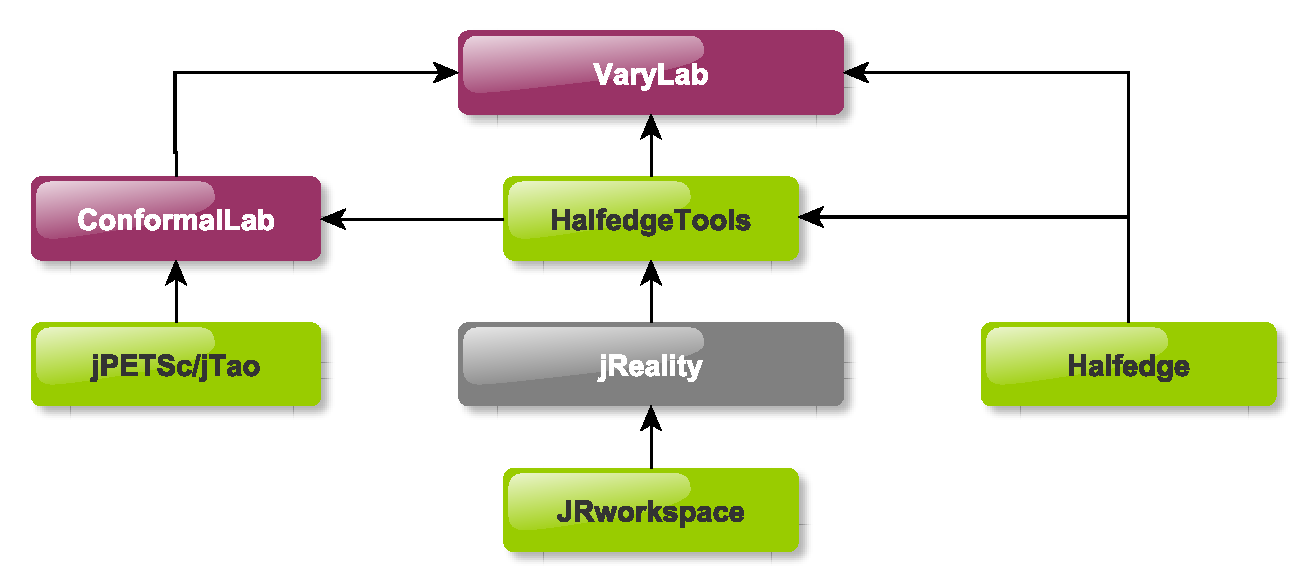
\includegraphics[width=\linewidth]{figures/software_architecture}
	\caption[Software package dependencies]{
		Software architecture and dependencies of the DDG Framework. 
		{\sc Jtem} library packages (green), mathematical software packages (red).
	}
	\label{fig:software_architecture}
\end{figure}

In the field of Discrete Differential Geometry (DDG) there is a special need for experiments
conducted with the help of computer software. Especially if the methods of DDG are applied
to problems in computer graphics, geometry processing, or architecture, algorithms have 
to be implemented and convincing examples have to be presented. Additionally a suitable 
visualization of the results has to be included in a state-of-the-art publication.

There is a growing knowledge of software development in the mathematical community. This 
is partly due to the curricula of universities which started to include programming courses for 
undergraduate students. {\bf [Find Reference ??]}
This enables the students to extend their abilities of creating visualizations and mathematical software, where former generations of students solely 
used the visualization abilities of standard computer algebra packages like Mathematica or MatLab.

This Chapter is the description and getting-started manual of a set of software packages
(Berlin DDG Framework) written in Java. They are specifically designed for the creation of
custom interactive software for experiments with algorithms and geometries treated 
within DDG. Section~\ref{sec:jrworkspace} introduces the {\sc JRworkspace} library of the 
{\sc Jtem} project~\cite{JtemWebsite}. It is the foundation of any application created with 
the DDG Framework. It is also the user interface basis of {\sc Jreality}, a mathematical 
visualization library that uses {\sc JRworkspace} as plug-in and user interface 
tool~\cite{JrealityWebsite}. Section~\ref{sec:halfedge_halfedgetools} introduces the 
{\sc Halfedge} and {\sc HalfedgeTools} package. It implements a half-edge data 
structure and various user interface tools and algorithms for interaction and editing.  
In Section~\ref{sec:conformallab} we describe the software 
{\sc ConformalLab}. This package implements the methods of the 
publications~\cite{Bobenko2010, OWR2012, Sechelmann2012, BobSechSpr}.
Section~\ref{sec:varylab} introduces {\sc VaryLab} the software implementation of the 
methods described in the publications \cite{Lafuente2011, Lafuente2012, Sechelmann2012}.
This package is also released to partners of the development group as 
{\sc VaryLab[Gridshells]}, {\sc VaryLab[Ultimate]}, or even online as {\sc VaryLab[Service]}.


Figure~\ref{fig:software_architecture} shows the dependencies of the packages. Every
application depends on {\sc JRworkspace} which implements plug-in functionality. It is
the basis of the {\sc Jreality} plug-in system. {\sc Half\-edge\-Tools} is using {\sc Jreality} 
for visualization and is build on top of the {\sc Jtem} project {\sc Half\-edge}. 
{\sc ConformalLab} and {\sc VaryLab} use {\sc Jpetsc/Jtao} to perform numerical
optimization. Their algorithms are implemented as {\sc JRworkspace} plug-ins.


The development of the described software is joint work with Thilo R{\" o}rig 
({\sc HalfedgeTools, VaryLab}), the {\sc Jreality} members~\cite{JrealityWebsite}, Hannes 
Sommer ({\sc Jpetsc/Jtao})~\cite{jpetsctao-web-page}, Ulrich Pinkall and Paul Peters ({\sc JRworkspace}), and 
Boris Springborn ({\sc Halfedge}).



\section{{\sc JRworkspace} - A Java API for modular applications}
\label{sec:jrworkspace}

\begin{figure}
	\centering
	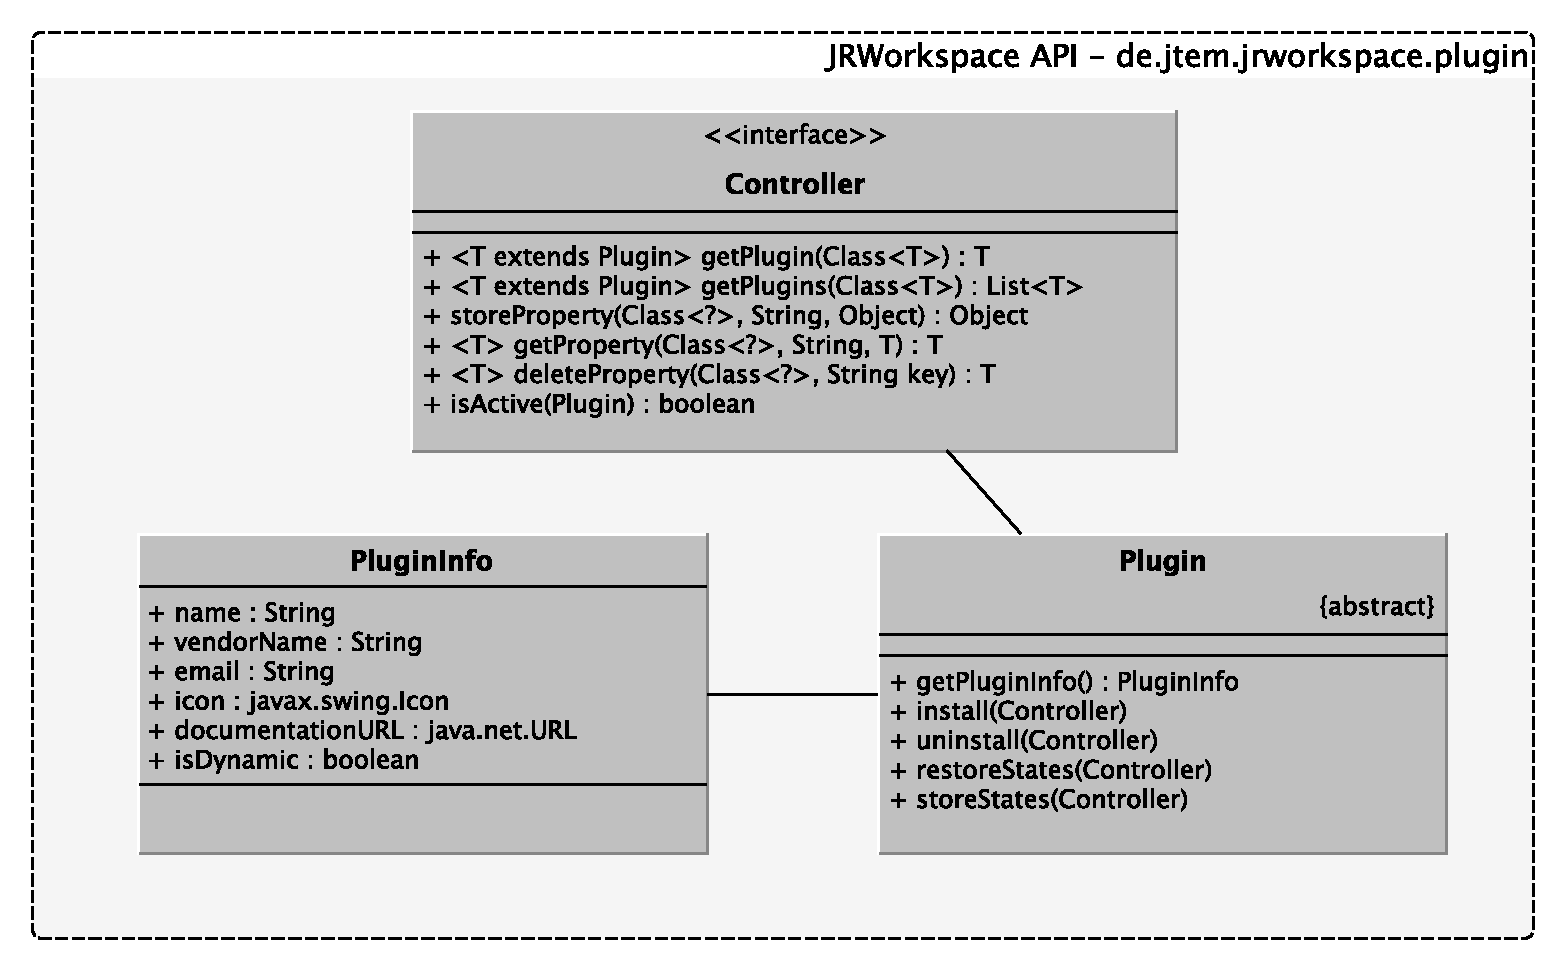
\includegraphics[width=0.8\linewidth]{figures/jrworkspace_uml}
	\caption[{\sc JRworkspace} API]{
		UML diagram for the {\sc JRworkspace} API.
	}
	\label{fig:jrworkspace_uml}
\end{figure}

The library package {\sc JRworkspace} is part of the {\sc Jtem} family of software projects \cite{JtemWebsite}. It defines a simple API to create modular Java applications. Figure~\ref{fig:jrworkspace_uml} shows the UML class diagram of the three main classes.
The project contains a reference implementation that supports the creation of Java
Swing applications. This implementation is used in all applications described in this work.

\subsection{Plug-ins}

\begin{table}
\centering
\begin{tabular}{r|r|l}
	{\tt restoreState} & 1. & load plug-in state values from Controller\\
	{\tt install} & 2. & calls getPlugin to obtain other plug-ins\\
	{\tt --}  & 3. & program execution\\
	{\tt storeStates} & 4. & stores state values in the Controller\\
	{\tt uninstall}/program terination & 5. & clean up
\end{tabular}
\caption{{\sc JRworkspace} plug-in life cycle}
\label{tab:plugin-lifecycle}
\end{table}

In {\sc JRworkspace} a module is called plug-in and extends the abstract class Plugin
(Figure~\ref{fig:jrworkspace_uml}). The idea is that a plug-in can be installed by the controller calling its {\tt install} method or uninstalled via
the uninstall() method. Before installation of a plug-in the controller calles the
{\tt restoreStates} method of a plug-in. The {\tt storeStates} method is called at program termination or right before uninstall of the plug-in.
Inter-plug-in-communication is done via the {\tt getPlugin} method of the controller. A plug-in should call {\tt getPlugin} from within the install method to obtain an instance of a dependent plug-in. See Table~\ref{tab:plugin-lifecycle} for the plug-in life-cycle.

\lstinputlisting[
	caption={A simple plug-in class. It depends on a plug-in called {\tt DependentPlugin} and has the property {\tt doubleState}. It provides the method {\tt doWork} that prints some message.}
       \label{lst:javaclass},
	captionpos=b,
	language=JAVA,
	firstline=6
] {java/de/sechel/thesis/MyPlugin.java}


\subsection{A reference implementation}



\subsection{Gui elements}
\subsection{{\sc JRworkspace} and {\sc Jreality}}
\subsection{Building a {\sc JRworkspace} application}

\section{The {\sc Jtem} libraries {\sc Halfedge} and {\sc HalfedgeTools}}
\label{sec:halfedge_halfedgetools}
\subsection{The halfedge data structure and tools}
\subsection{Data model and algorithms}

\section{{\sc ConformalLab} - Conformal maps and uniformization}
\label{sec:conformallab}
\subsection{Embedded surfaces}
\subsection{Elliptic and hyperelliptic surfaces}
\subsection{Schottky data}
\subsection{Surfaces with boundary}

\section{{\sc VaryLab} - Variational methods for discrete surfaces}
\label{sec:varylab}
\subsection{Functional plug-ins}
\subsection{Implemented functionals and options}
\subsection{Remeshing}

\section{{\sc U3D} - 3D content in presentations and online publiciations}
\label{sec:u3d}
\subsection{3D content in PDF documents}

\section{Non-linear optimization with {\sc Jpetsc/Jtao}}
\label{sec:jpetsctao}
\subsection{A java wrapper for {\sc Jpetsc/Jtao}}

%%% Local Variables:
%%% TeX-master: "Thesis.tex"
%%% End: